\section{Scripting with EASE}
In addition to interacting with tools via the ICE user interface, ICE also
provides a scripting framework based on the Eclipse Advanced Scripting
Environment (EASE). 

\subsection{PyDev Installation (optional)} 

Although it is possible to edit Python scripts in Eclipse using the default text editor,
however it is much more productive to use the PyDev Eclipse development
environment if you are planning to do a lot of script development. In addition to the 
usual syntax coloring and other advanced editing features you'd expect in Eclipse, 
PyDev also provides the ability to run and debug Python programs from within the Eclipse environment.

PyDev can be easily installed from using the Eclipse Marketplace client as
follows. From the ICE menu bar, select \texttt{Help $\rightarrow$ Eclipse
Marketplace\ldots}, type ``pydev'' in the Find field, then click the \texttt{Go}
button.
After a few seconds, you should see an entry for PyDev as shown in figure
\ref{fig:pydev}.
Simply click the \texttt{Install} button and follow the prompts to install the feature. Once
Eclipse has been restarted, any Python scripts ending in ``.py'' will be recognized by
PyDev and opened in the Python editor by default.

\begin{figure}[!ht]
\centering
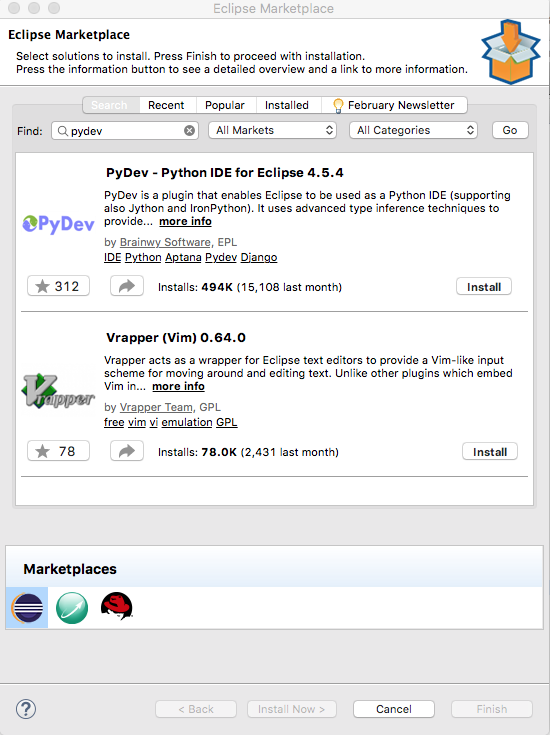
\includegraphics[width=8cm]{images/pydev-marketplace}
\caption{Installing PyDev}
\label{fig:pydev}
\end{figure}

\subsection{EASE Configuration}

There are a number of configuration settings that can be used to customize the
behavior of EASE. These configuration settings are accessed via the \texttt{Scripting}
preference page in the Eclipse preferences. To open the \texttt{Scripting}
preference page, select \texttt{Window $\rightarrow$ Preferences\ldots} in the
ICE menu bar. (On Mac OS X, Preferences\ldots is instead located under Eclipse
ICE in the menu bar.) Open the \texttt{Scripting} tree item on the left side of
the preferences window and you will see the different preferences that can be
configured.

\begin{figure}[!ht]
\centering
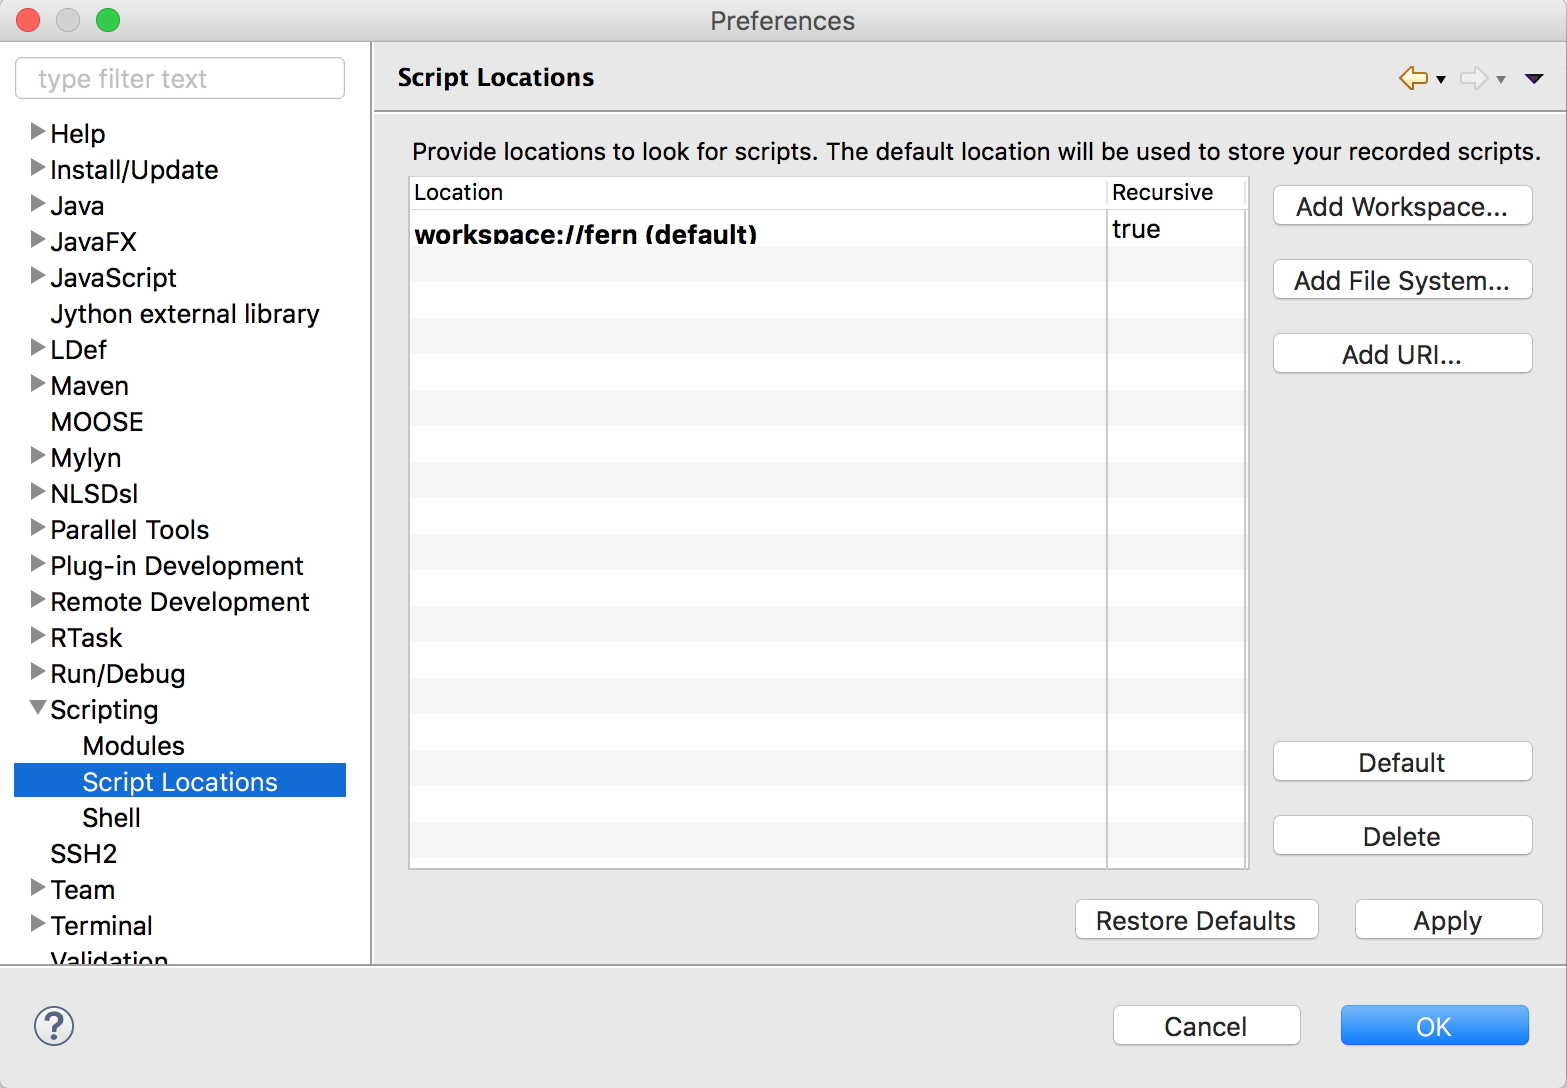
\includegraphics[width=8cm]{images/scripting-prefs1}
\caption{Setting the Script Locations}
\label{fig:prefs1}
\end{figure}

EASE works best if you keep your scripts in one or more projects in
your workspace. You can then associate these \emph{Script Locations} so
that EASE knows they are used for managing your scripts. You can either use an
existing project, or create a new project for the scripts. In this tutorial,
we're just going to use the existing \texttt{itemDB} project to store our scripts, but
you could just as easily create a new one. To configure the projects, select the
\texttt{Script Locations} preference item to reveal the dialog shown in figure
\ref{fig:prefs1}. You can then use the \texttt{Add Workspace\ldots} button to
select one or more projects from the workspace.

By default, EASE is configured to use the JavaScript (Rhino) engine.
Since this tutorial assumes that the preferred environment is Python, we recommend changing
this default. To set the script engine default, select the
\texttt{Shell} preference item. Next, select \texttt{Python (Jython)} from
the \texttt{Preferred Engine:} dropdown as shown in figure \ref{fig:prefs2},
then click on \texttt{OK}.

\begin{figure}[!ht]
\centering
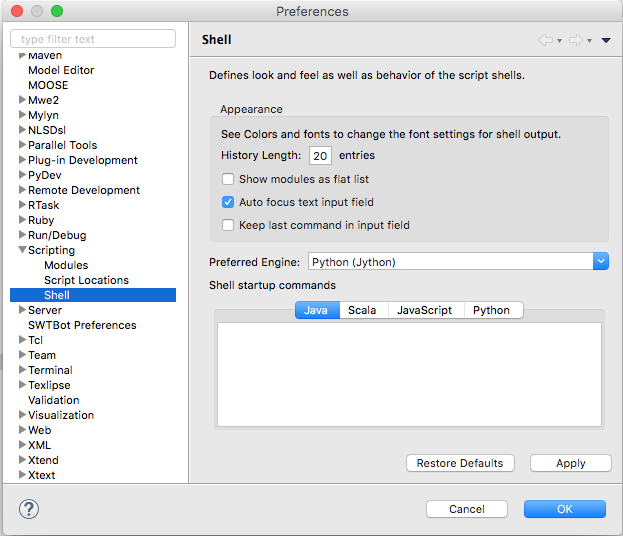
\includegraphics[width=8cm]{images/scripting-prefs2}
\caption{Setting the Default Engine}
\label{fig:prefs2}
\end{figure}

\subsection{Creating and Running Scripts}

There is nothing special about creating and running EASE scripts. They can be
created in a variety of ways using the development tools available in ICE, and
then run later when needed. For this tutorial, we will be creating the scripts
using PyDev (or any text editor) and running them directly using the \texttt{Run As
$\rightarrow$ EASE Script} context menu.

EASE also provides a perspective for creating, managing, debugging, and running
scripts called the \texttt{Scripting} perspective. This perspective contains
views for running script commands interactively, and for exploring script modules.
To switch to the \texttt{Scripting} perspective use the \texttt{Perspective
Switcher} icon or select the \texttt{Window $\rightarrow$ Perspective
$\rightarrow$ Open Perspective $\rightarrow$ Other\ldots} menu, then select 
\texttt{Scripting} from the list. You should see the perspective shown in figure
\ref{fig:perspective}.

\begin{figure}[!ht]
\centering
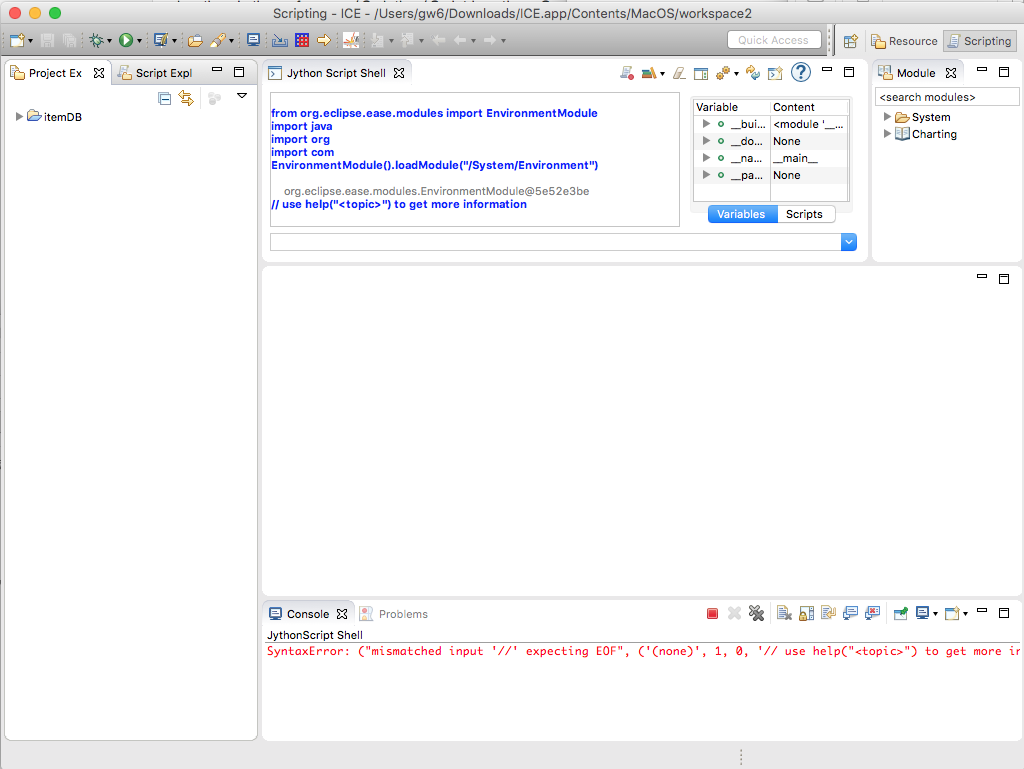
\includegraphics[width=\textwidth]{images/perspective.png}
\caption{Scripting Perspective}
\label{fig:perspective}
\end{figure}

EASE hides many of the details that would normally be required to manipulate
Java objects and perform actions in the Eclipse IDE. It does this by
encapsulating typical actions into simple script commands that can be easily
invoked from scripts that you write. These commands are collected together into
``modules''. You can see which modules are available, and the commands that they
contain, using the \texttt{Modules Explorer} view. This view is visible in
the top right corner of the \texttt{Scripting} perspective. The \texttt{Modules
Explorer} view can also be opened by selecting \texttt{Window $\rightarrow$ Show
View $\rightarrow$ Other\ldots} to open the \texttt{Show View} dialog, the open
the \texttt{Scripting} folder and select the \texttt{Modules Explorer} and click
on \texttt{OK}.

\subsection{Creating a Python Script}

The easiest way to create a Python script is to simply create a text file ending
in ``.py'' in an existing project. If your scripts will be used with stand-alone Python
programs, you can use PyDev to create a Python project, but in general, any kind
of project will suffice.

For this tutorial, we're going to use the \texttt{itemDB} project that has
already been created, and should be visible in the \texttt{Project Explorer}
view. You can now create a Python file in this folder by right clicking on the
folder and selecting \texttt{New $\rightarrow$ File} from the context menu. 
This will display the \texttt{New File} dialog as shown in figure \ref{fig:newfile}.

\begin{figure}[!ht]
\centering
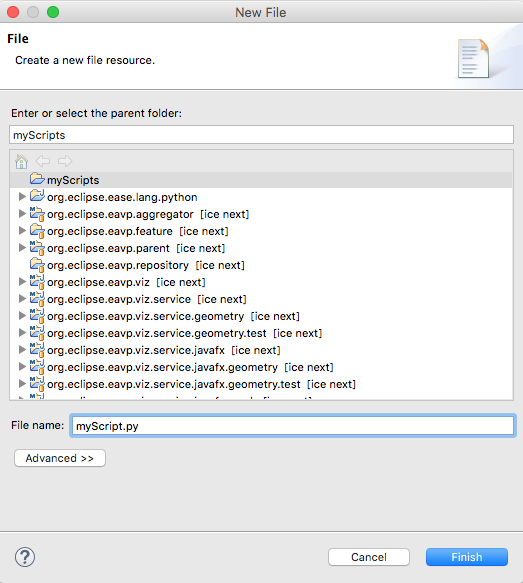
\includegraphics[width=8cm]{images/newfile}
\caption{New File Dialog}
\label{fig:newfile}
\end{figure}

At this point all that remains to be done is enter the name of the file in the
\texttt{File name:} field and click on the \texttt{Finish} button. This will
create the file and automatically open the PyDev editor (assuming you installed
PyDev) or a simple text editor. You should see an editor view something like
that shown in figure \ref{fig:editor}.

Since the \texttt{itemDB} project was selected as a scripting location
previously, the new script file should also be visible in the \texttt{Script
Explorer} view in the \texttt{Scripting} perspective. Make sure the
\texttt{Scripting} perspective is selected for this view to be visible.

\begin{figure}[!hb]
\centering
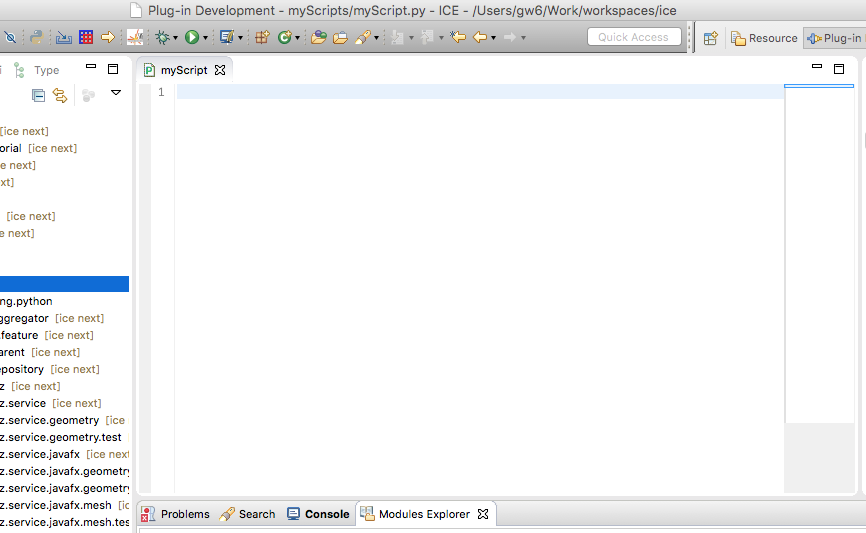
\includegraphics[width=8cm]{images/editor}
\caption{Editor View}
\label{fig:editor}
\end{figure}


\subsection{Writing a Python Script}

Our first python script will just print ``Hello World'' on the console. Enter
the following text in the editor and select \texttt{File $\rightarrow$ Save}:

\begin{verbatim}
print 'Hello World'
\end{verbatim}

Once you have entered the Python script, is can be easily launched using the run
button (green arrow) on the \texttt{Script Exporer} view. Simply select the
the script file you want to run and click on the run button. Any (textual)
output generated by the script will be displayed in the Console view shown in
figure \ref{fig:console}.

\begin{figure}[!ht]
\centering
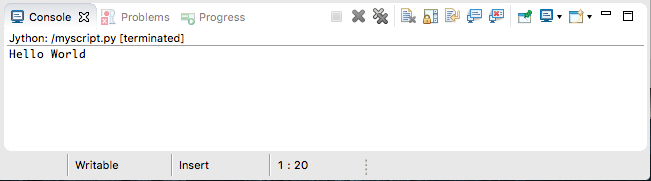
\includegraphics[width=10cm]{images/console}
\caption{Console View}
\label{fig:console}
\end{figure}

Rather than using the run button, we would like to run this script using our own
button on the \texttt{Project Explorer} view. To do this, add the following
lines to the start of the script, then save the file:

{\small
\begin{verbatim}
# ********************************************************************  
# name                 : My Script 
# toolbar              : Project Explorer  
# script-type          : Python  
# description          : Start a file browser using current selection.  
# ******************************************************************** 
\end{verbatim}
}

As soon as you save the file, you should notice a couple of things. The name of
the script file will change to \texttt{My Script} in the \texttt{Script
Explorer} view, and if you switch to the \texttt{Project Explorer} view, you
should see a \texttt{My Script} button in the view toolbar (as shown in figure
\ref{fig:myscript}).

We can modify the user interface behavior by changing the button to an icon and
adding a popup conext menu. This is accomplished by adding the following lines
to the script:

{\small
\begin{verbatim}
# popup				   : enableFor(org.eclipse.core.resources.IResource) 
# image				   : platform:/plugin/org.eclipse.ui.ide/icons/full/elcl16/configs.png
\end{verbatim}
}

\begin{figure}[!ht]
\centering
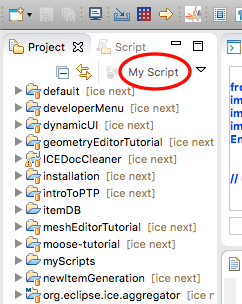
\includegraphics[width=6cm]{images/projexplorer}
\caption{New Button in Project Explorer view}
\label{fig:myscript}
\end{figure}

\subsection{Interacting with ICE}

In order to interact with Java classes in ICE from the Python script, we 
need to include the \texttt{Platform} module. In order to load a module, we use
the \texttt{loadModule()} function in Python. The argument to this function is a
string representation of the module path, which in this case will be
\texttt{/System/Platform}. 

In the \texttt{Modules Explorer} view, open the \texttt{System} folder, then drag
the \texttt{Platform} item onto first line of the script file. This should insert
the following line into your script:

\lstset{basicstyle=\ttfamily\small, breaklines}

{\small
\begin{verbatim}
loadModule("/System/Platform")
\end{verbatim}
}

Once this module has been loaded, a number of additional functions become
available. We want to obtain a reference to the core ICE service, which is used
as the starting point for manipulating ICE models. This is done by adding the
following line:

{\small
\begin{verbatim}
coreService = getService(org.eclipse.ice.core.iCore.ICore)
\end{verbatim}
}

Once a reference to the core services has been obtained, we can use this to
obtain a reference to the Reflectivity Model and set some parameters. This is
done by adding the following lines:

{\small
\begin{verbatim}
reflectModel = coreService.getItem(int(coreService.createItem("Reflectivity Model")))
component = reflectModel.getComponents().get(0)
entry = component.retrieveAllEntries().get(0)
entry.setValue("waveVector_space.csv")
\end{verbatim}
}

Note that the \texttt{createItem()} method will return a string representing the
number of that item, so \texttt{int()} is used to convert it to an integer, which is the
argument expected by \texttt{getItem()}.

Now the only thing left to do it process the model. This is done using the core
service \texttt{processItem()} as follows:

{\small
\begin{verbatim}
res = coreService.processItem(reflectModel.getId(), "Calculate Reflectivity", 1)
\end{verbatim}
}

Finally, let's print out the result of processing the model to see if it was
successful.

{\small
\begin{verbatim}
print "result was: %s" % res
\end{verbatim}
}

Remember to save the editor using \texttt{Ctrl/Cmd-S} or the \texttt{File
$\rightarrow$ Save} command from the ICE menu bar.

Before running this script, you need to copy the \texttt{waveVector\_space.csv}
file from the \texttt{default} folder to the \texttt{itemDB} folder. You should
then be able to run the script successfully.

\subsection{Using the Sample Scripts}

\lstset{basicstyle=\ttfamily\scriptsize, breaklines}
\makeatletter
\def\lst@lettertrue{\let\lst@ifletter\iffalse}
\makeatother

We have provided a number of sample scripts to show how ICE can be
scripted using EASE.
These scripts are located in the
\path{org.eclipse.ice.examples.reflectivity} package that is already loaded
in your workspace. The scripts can also be obtained by cloning the ICE Git
repository\footnote{\texttt{http://github.com/eclipse/ice.git}},
then manually importing the \path{org.eclipse.ice.examples.reflectivity}
package.

There are four sample scripts that demonstrate how a reflectivity model
can be created, configured and executed. The scripts are described in
more detail in the following sections.

\subsubsection{createAndProcessPython.py} 

This is a simple script
that demonstrates how to create a reflectivity model and process the model to
obtain a result. The default model inputs are used for the computation.

\lstinputlisting[language=Python]{samples/createAndProcessPython.py}

\subsubsection{createAndEditPython.py} 

This script extends the
\texttt{createAndProcessPython.py} script by editing the input to the model
programmatically. The model is then processed to obtain the results.

\lstinputlisting[language=Python]{samples/createAndEditPython.py}

\subsubsection{iterateChangeParameterPython.py} 
This script demonstrates how to create
multiple reflectivity models with varying input parameters. The models are created
and processed sequentially.

\lstinputlisting[language=Python]{samples/iterateChangeParameterPython.py}

\subsubsection{listFromScratchPython.py} 
This script demonstrates how to create a
reflectivity model and programmably create and set up the layers in the model.
The model is then process to obtain the results.

\lstinputlisting[language=Python]{samples/listFromScratchPython.py}
